% Test

\chapter{Test and Test setup} % Main chapter title

\label{Test} % For referencing the chapter elsewhere, use \ref{method} 

%----------------------------------------------------------------------------------------
The Long Term Reliability Testing (LTRT) of ATLAS ITk modules is intended to be conducted through a systematic approach aimed at evaluating their performance under various conditions. In this section, we will introduce the test setup and the test software and controls in detail, and outline and provide an explanation of each test performed during a full cold LTRT.\\

\section{Test Setup}

The test setup designed for thermal cycling and long-term reliability testing is specialized equipment that can maintain an environment with temperature and humidity controlled for testing the performance of detector components. \textcolor{blue}{In addition to that, it provides an isolated environment to prevent unwanted photons and electromagnetic noises disturb the test.} This equipment, known as "Coldbox", typically have the capability to reach and maintain a range of low temperatures. This temperature range is chosen to simulate the operating conditions of the detector, which is chosen because the noise is significantly reduced at this temperature. In addition to the temperature, Coldbox regulates and monitors several environmental parameters such as relative humidity, airflow, and dew point, and is also able to control temperature for each installed module. Fig.\ref{fig:coldbox} shows an overview of the equipment. \\

\begin{figure}[h]
    
    \begin{subfigure}[b]{0.45\textwidth}
        \centering
        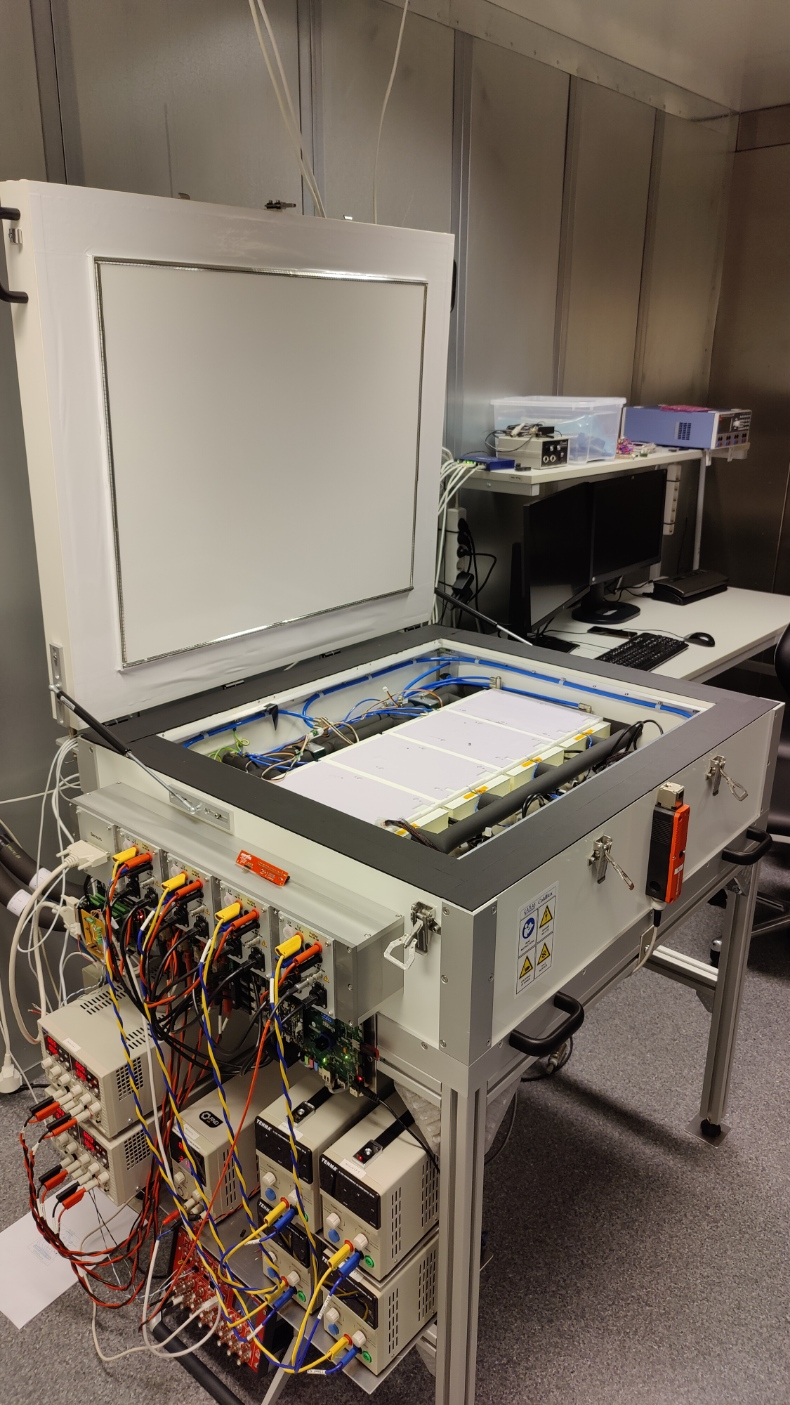
\includegraphics[width=7cm,height=8cm,keepaspectratio]{Figures/test/coldbox-1.jpg}
        \caption{}\label{fig:coldbox1}
    \end{subfigure}
    ~
    \begin{subfigure}[b]{0.45\textwidth}
        \centering
        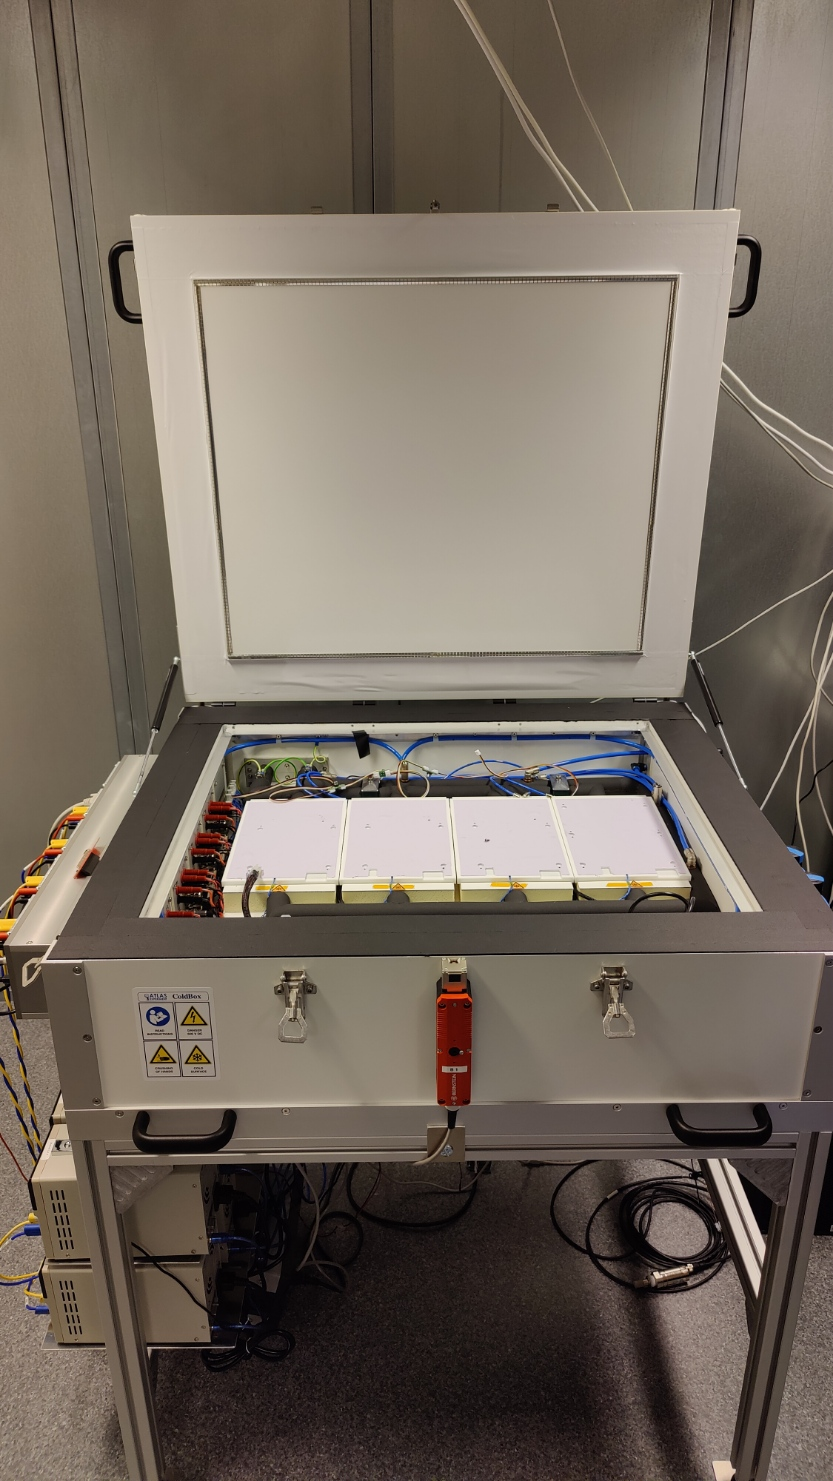
\includegraphics[width=7cm,height=8cm,keepaspectratio]{Figures/test/coldbox-2.jpg}
        \caption{}\label{fig:coldbox2}
    \end{subfigure}
    \caption{An overview of the Coldbox from a) front view, and b) side view, showcasing the general properties of the equipment and connected devices and sensors.}
    \label{fig:coldbox}
\end{figure}

\subsection{Coldbox}
The long-term reliability testing is conducted under a regulated setting with a fixed temperature of $-35\si{\celsius}$, \textcolor{blue}{but for the proof of concept intended for this work, and reduce the temperature regulation time, the tests are conducted at $0\si{\celsius}$.} The environmental parameters are monitored and maintained constant by the Coldbox throughout the duration of the test (Active and IDLE). The temperature of each module is controlled zonally by $4$ "chucks", on which one module can be installed. Heat sinks attached to a chiller and "Peltier" components are positioned on each chuck to allow the temperature of the modules to be precisely changed and set on demand.\\

Coldbox is equipped with four different types of power supplies: $4$ individual Low Voltage (LV) power supplies, responsible for powering each installed module, a High Voltage (HV) power supply, to inject the test charge to the modules, $4$ individual power supplies to heat up the Peltiers separately (Fig.\ref{fig:supplies}), and one power supply to power the airflow system, RaspberryPi board, interlock, and by-pass valves. The operating voltage of the modules is typically $\approx 11 \si{\volt}$. The HV power supply, on the other hand, delivers up to $500 \si{\volt}$ for the purpose of these tests (bias of $-500 \si{\volt}$). The operating voltage of the Peltiers' power supplies varies by the set temperature.\\

The box is cooled down to $30\si{\celsius}$ by an external chiller, using silicone oil as the coolant, and maintains the temperature of the Coldbox at a desired level during the tests. \textcolor{blue}{The exact desired temperature then is set by the Peltiers, which can increase or decrease the temperature of the module with great precision (Fig.\ref{fig:cooling}). The reason for this configuration is that first, as mentioned, the chiller cannot regulate the temperature årecicely as needed during the test, and second, pushing the peltiers to achieve to low temperature requires a great amount of current provided in a short time, which will cause serious issue to them.}\\
In addition to the above, the airflow is controlled \textcolor{red}{WHY?} and maintained using a flow control valve and a digital flow meter (Fig.\ref{fig:airflow1} to \ref{fig:airflow3}). \\

Outside the box, 3 different controller boards are installed; a RaspberryPi board running coldjiglib which is the commanding unit of the Coldbox, \textcolor{blue}{a polarity switch that is responsible for alternating the current of the Peltiers}, and a data collection unit that holds 4(+1) data ports, each for one module (Fig.\ref{fig:connections})\\

The relative humidity on each module is measured using a humidity sensor. These sensors are installed at the end of the outlet flow connection, and read the humidity of the flown air inside the installed module's casing. Using the relative humidity and the temperature of the air on each module, we can calculate the dew point using Eq.\ref{eq:dewpoint}. \textcolor{blue}{These measurements, and the dew point value, in particular, are crucial to preventing the formation of water droplets on the electronic components.}\\

\textcolor{blue}{Lastly, the box is secured and locked by an interlock system, to implement safety measurements due to the high voltage presence during the tests}, as well as to prevent unwanted access to the box during the tests and exposure of the modules to the ambient environment. \footnote{for more information please refer to \textcolor{red}{EDU's Thesis}.} (Fig.\ref{fig:interlock}).\\


\subsection{Test Software and Controls}
The configuration of the modules, calibrations, tests, and data collection from the tests are handled by the ITk Strip Data Acquisition (ITSDAQ) software developed by the strip community. After installation of the modules, each module depending on the type needed to be introduced to ITSDAQ in order to get the correct module configurations. Each LTRT test starts with a "Pre-Test" procedure, which acquires an IV test before powering on the hybrid (\textbf{WHY??}), and then, the hybrid is powered and the cooldown procedure is initiated. \textcolor{blue}{As the ColdBox regulates the environmental parameters, and it reaches to the desired cold temperature}, the high voltage is injected, and subsequently, the ABCstar full test is run. This procedure is repeated between pre-set intervals (typically every 12 hours for LTRT, \textcolor{blue}{but for the purpose of this work in very short intervals of 10 to 15 minutes}), for a required number of instances. \\

\textcolor{blue}{To ensure traceability during HL-LHC operation and subsequent stages of manufacture, it is imperative to record and preserve data from the QA/QC of each individual module. As more testing facilities are assigned for conducting LTRT and thermal cycling tests, it's critical to store test results in an international database for future analysis. In addition to the test results provided by ITSDAQ, and in order to validate the stability of the Coldbox and track down any potential abnormality in the test results of the modules, it is crucial to record and monitor the environmental and electrical data during the tests.} \\

\textcolor{blue}{Along with the above-mentioned considerations, another issue that needed to be taken into account was keeping these records safe and keeping them in a central database for upcoming research and studies. To address this problem and work with other testing facilities, we store all of the environmental, AMAC, and electrical test data along with the related metadata in different datasets. We then use the process that has been put into place to upload the data to a central database.}\footnote{\textcolor{blue}{The implemented procedure also captures the electrical data from the power supplies during normal operation, but during the development stage, this data is not returned by the software.}} Fig.\ref{fig:testworkflow} shows an overview of the workflow between different components of the test and the pathway of each relevant data to the database. 

\begin{figure}[h]
    \centering
    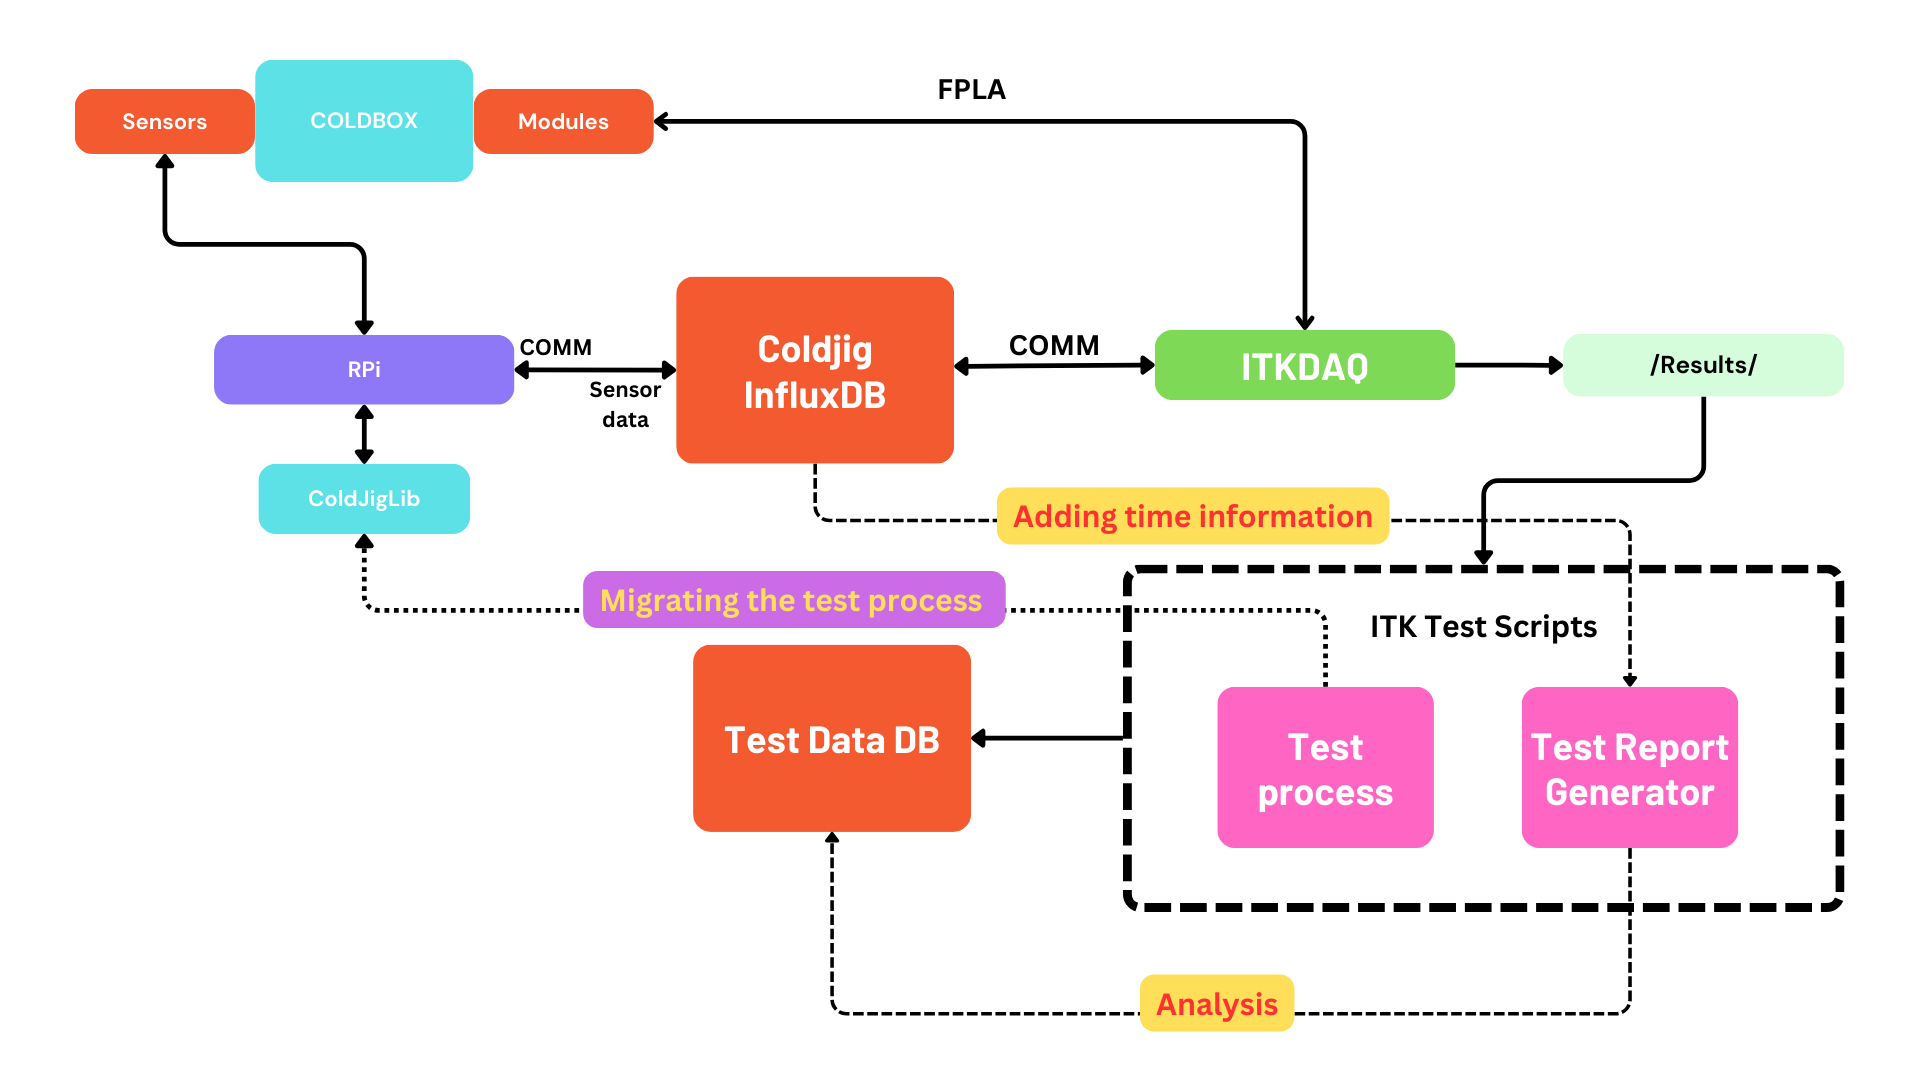
\includegraphics[width=10cm,height=11cm,keepaspectratio]{Figures/test/test diagram2.png}
    \caption{A diagram of the workflow of the LTRT test, from the start of the test}
    \label{fig:testworkflow}
\end{figure}

\subsection{The Environmental Data}
While ITSDAQ is essential for gathering and processing data from the ATLAS ITk modules, environmental data collection is not included in its scope. However, the integration of environmental data is crucial for a complete analysis and understanding of the modules' functionality. Temperature, dew points, relative humidity, and other variables can have a big impact on the behavior and dependability of modules. To accommodate these parameters, it is needed to retrieve data directly from the ColdBox and integrate it with the analyzed data from ITSDAQ. The ColdJiglib as the running heart of the Coldbox, enables us to gather environmental data. \\

As explained in the previous part, several LTRT tests are performed within a set time interval. Each test is tagged by the number of iterations and is presented by InfluxDB. To get access to the environmental data, we implemented a series of logics and queries, which find the latest test performed by presenting the test file, and find the time intervals in which the module was kept in the controlled environment (IDLE state) and the time interval that the LTRT is performed. The data is then stored in datasets with related metadata in order to be uploaded to the test database. \textcolor{blue}{ Afterwards, and for analytical purposes, we can compare the timestamps given by the environmental data and the test results, and we can examine the behavior of the module during the test in conjunction with the environmental data.}


\subsection{The Electrical Data}
In addition to the environmental data from the Coldbox, electrical data from the AMAC and the HV power supply needs to be monitored.\textcolor{blue}{ The AMAC data offers insightful information on how well the detector system is operating. Through the process of monitoring voltage levels, current consumption, and temperature, we are able to evaluate the general condition and operation of the detector components. It is important to mention that the AMAC individually records separate measurements of the temperature on each hybrid and the power board, as well as the voltage, current, and calibration parameters. Table \ref{tab:AMAC_params} enlisted the details of the measurement and parameters from AMAC.} 


\subsection{Physics behind the tests}
The tests (as we will be explained elaborately) are designed to characterize the electrical properties and performance of the ITk modules, particularly to determine the qualitative performance and endurance of the modules during the commissioning time. Several physical concepts are involved within the tests, that need to be explained before digging deep into the tests and their results. 

\subsubsection{Occupancy}
In the context of silicon detectors, occupancy refers to the fraction of detector elements that register a particle interaction within a specific time frame. It's essentially a measure of how "busy" the detector is. A high occupancy rate indicates a high level of particle activity or radiation in the detector, which can affect its ability to accurately measure particle tracks, identify particles, and distinguish between signal and background. Fig.\ref{fig:occupancy} illustrates the detection of particles in high and low occupancy situations.


\begin{figure}[h]
    \centering
    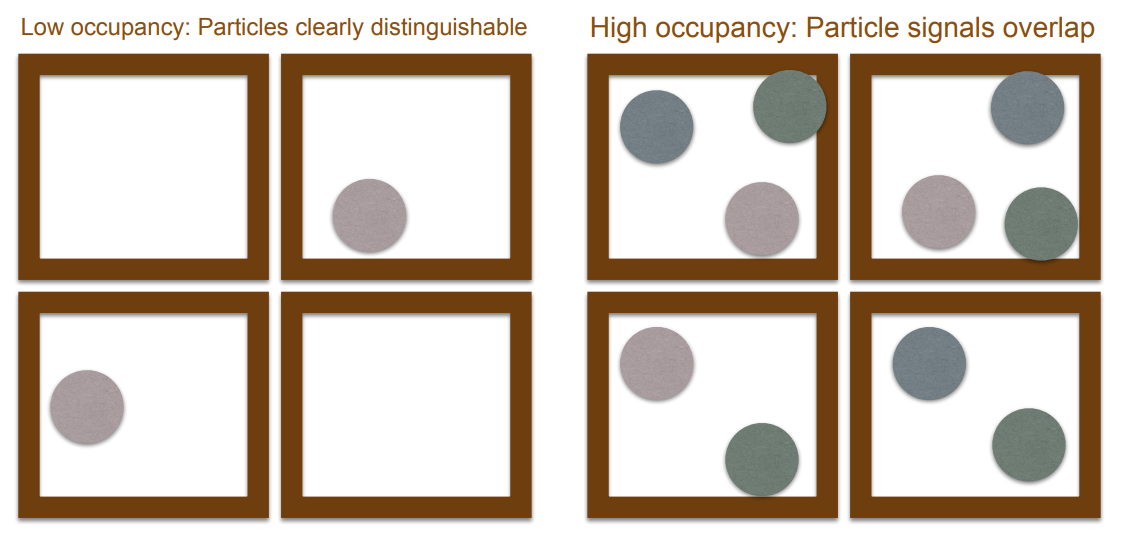
\includegraphics[width=8cm,height=7cm,keepaspectratio]{Figures/modules/occupancy.PNG}
    \caption{The schematic view of the detection of the particles by the silicon detector with a) low occupancy (left), and b) high occupancy(right)\cite{materClassDetection}.}
    \label{fig:occupancy}
\end{figure}

\subsubsection{Gain}
As explained in the previous part, the particles moving across silicon strips produce electric signals that are amplified and digitized, in order to be read-out. The process where the detector amplifies the signal generated by a particle interaction is referred to as gain. 
Due to the intrinsic voltage differential across the junction, when a particle interacts near it, the electric field accelerates the generated charge carriers across the junction, resulting in the creation of an extra current component. The overall signal may be improved by this additional current \cite{barr}.


\subsubsection{Threshold (Voltage threshold)}
\begin{wrapfigure}{r}{7cm}
    \centering
    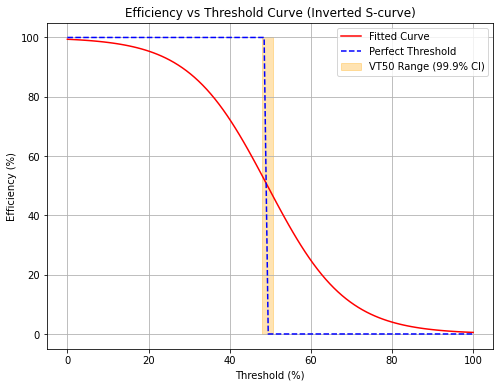
\includegraphics[width=7cm,height=7cm,keepaspectratio]{Figures/modules/threshold.png}
    \caption{A demo plot of the efficiency of the detection versus the threshold voltage (percentage from minimum to maximum operation voltage) showcasing the fitted curve and a perfect threshold.}
    \label{fig:threshold}
\end{wrapfigure}
The lowest voltage level required for generating a response or detection from the sensor or detector system is referred to as the voltage threshold. The voltage threshold is typically used for the response curve and during the test, to find the point at which the detector starts to consistently detect or respond to incoming signals, the voltage threshold is usually adjusted. The lowest signal amplitude or energy level that the detector is capable of accurately detecting and measuring is represented by this threshold voltage. But in practice, this minimum voltage is not a cut in the response, but a range in which the response is optimum, and within the ITk dictionary is referred to as "Vt50".  In other words, "Vt50" refers to the threshold voltage at which a detector channel detects or responds to a signal with a $50\%$ probability. During the test, since we do not deal with the actual charged particles, the signal is a $1 \si{\femto\coulomb}$ injected charge introduced to the sensor. Fig.\ref{fig:threshold} shows a demonstration of the threshold selection. As shown in the figure, there is an area where the sensor detection is optimum. This area, which is shown in yellow, can be considered as noise. 

\subsubsection{Noise}
Unwanted electrical signals or fluctuations that may interfere with accurate particle signal identification and measurement are referred to as noise. The detector's performance may be impacted by noise, which can originate from a variety of sources within the electronics and detection system, and it can substantially reduce the signal-to-noise ratio, resulting in a lower detector performance. Fluctuations in the electronic components and circuitry of the detector's readout (Electronic noise), electromagnetic and radiofrequency interference (Environmental noise), and leakage currents, capacitance variations, and fluctuations in the semiconductor properties (Densor noise), are some of the known and possible sources of noise in a silicon detector.\\
In the context of electronics and signal processing, typically two different noises are introduced: Input Noise, and Output Noise \footnote{In ITk databases and tests they are referred to as "innse" and "outnse", respectively}. The input noise is the noise introduced at the beginning of the signal chain, typically before any amplification or processing occurs, while the noise present in the signal after it has undergone amplification, processing, or other forms of manipulation within the system. By definition then, we can determine that the input noise is not directly measurable (or at least without using additional testing equipment), but from the processed signal which contains the output noise, and the gain, we can determine the input noise as:
\begin{equation*}
    \text{input noise} \cdot \text{gain} = \text{output noise}
\end{equation*}

\subsubsection{Dew point}
In addition to the tests, much of the environmental and electrical data is rather calculative, that measurement directly from the sensors. One of the most important of these types is Dew Point (DP). Assuming constant air pressure, the dew-point temperature is the lowest temperature at which saturation of the air can be reached. The relative humidity reaches $100\%$ when the temperature drops to the dew point, which can cause fog or dew. There are several formulations to calculate dew point, whether it is calculated by the pressure or temperature and relative humidity, but since in the context of our tests, The measurements are the air temperature and relative humidity,\textcolor{blue}{we use the following formula to calculate the liquid saturated water vapor pressure and through that the dew point. For the temperatures between $0\si{\celsius}$ to $200\si{\celsius}$ we have:}

\begin{equation}
    ln(P_{\text{water}}) = \sum_{i=-1}^3 (g_i T^{i}) + g_4 \ln_(T)
    \label{eq:lnvp}
\end{equation}

Where the coefficients are:
\begin{equation*}
    g_{-1} = \num{-5.800221e+03} \hspace{1cm}
    g_0 = \num{1.391499e+00} \hspace{1cm}
    g_1 = \num{-4.864024e-02}
\end{equation*}

\begin{equation*}
    g_2 = \num{4.176477e-05} \hspace{1cm}
    g_3 = \num{-1.445209e-08} \hspace{1cm}
    g_4 = \num{6.545967e+00}
\end{equation*}

For the temperatures between $-100\si{\celsius}$ to $0\si{\celsius}$ we have:
\begin{equation}
    ln(P_{\text{ice}}) = \sum_{i=0}^5 (m_i T^{i-1}) + m_6 \ln_(T)
    \label{eq:lnvp}
\end{equation}

Where the coefficients are:
\begin{equation*}
    m_0 = \num{-5.674536e+03} \hspace{0.7cm}
    m_1 = \num{6.392525e+00} \hspace{0.7cm}
    m_2 = \num{-9.677843e-03} \hspace{0.7cm}
    m_3 = \num{6.221570e-07}
\end{equation*}

\begin{equation*}
    m_4 = \num{2.074783e-09} \hspace{1cm}
    m_5 = \num{-9.484024e-13} \hspace{1cm}
    m_6 = \num{4.163502e+00} 
\end{equation*}


\begin{equation}
    P = exp(ln(P))
    \label{eq:ws}
\end{equation}

The dew point can be calculated as:
\begin{equation}
    DP(T, RH) = ws \cdot RH
    \label{eq:dewpoint}
\end{equation}

\textcolor{blue}{ Where $P_{\text{water}}$ is the saturation pressure of water vapor, $ws$ is the water saturation, $D_P$ is the dew point as a function of temperature and relative humidity, RH is the relative humidity, $T$ is the temperature. \cite{DPformula}. }



\section{ABCstar full test}
ITSDAQ, as explained above, is the mainframe for running the electrical tests for each installed module. For the reliability testing of the module, $4$ tests are conducted on the ABCstar chips, as listed below:

\subsection{Trim range test}
Trimming involves adjusting parameters such as voltage thresholds, current levels, gain settings, or other characteristics that influence the performance of the ABCstar. The goal of trimming is to ensure that the device operates within specified tolerances and meets performance requirements under various operating conditions.\\
The "Trim Range" test focuses on optimizing the trims within the chips to minimize response variations among channels. This test involves conducting a series of threshold scans with a fixed injected charge while adjusting the trim settings of the chips. The goal is to identify trim settings that produce a uniform response across all channels. The outcome of this test may result in identifying un-trimmable channels or chips, or it may yield the optimal trim settings for each channel.\cite{ARGOS2019112}

\subsection{Strobe delay test}
The Strobe Delay test involves adjusting the phase of the charge injection relative to the trigger signal. This means altering the timing or synchronization between when the trigger signal is sent to the circuit and when the charge injection occurs. By varying this phase, engineers can determine the optimal timing at which the injected pulses are most effectively detected by the circuit.\cite{ARGOS2019112}

\subsection{Response curve}
The Response Curve test is used to characterize the performance of the front-end electronics in detecting signals of varying amplitudes. We test the system with ten different signal strengths, from weak to strong. \cite{ARGOS2019112} Each response curve test consists of several steps: \\
\begin{itemize}
    \item Noise Measurement: measures the background electrical noise when no signals are present.
    \item Threshold Finding: For each signal strength, we find the point where the system detects half of the signals. This gives us a good idea of when the system starts picking up signals. The median point, denoted as $V_{t50}$, is extracted from each threshold scan. This median point represents the voltage threshold at which $50\%$ of the signal events are detected.
    \item Gain Calculation: Calculate how much the system amplifies the signals it detects. This tells us how sensitive the system is to weak signals. Using the ten $V_{t50}$ values obtained from the threshold scans, an exponential fit is performed to determine the gain of the front-end electronics.
    \item Input Noise Calculation:  Using the gain and noise measurements, we figure out how much random noise affects the system's ability to detect signals.
\end{itemize}

\subsection{Noise occupancy}
\textcolor{blue}{Noise occupancy represents the percentage of time that each channel registers noise events above a certain threshold level, and helps us to assess the level of background noise in the detection system. Several factors can affect noise occupancy such as the design of the readout electronics, the quality of signal processing algorithms, environmental conditions, and shielding against external noise. High noise occupancy, can negatively influence the detector performance due to the increased possibility of false positive readings and the decreasing signal-to-noise ratio.} \\

\subsection{I-V test}
The IV test allows us to measure the leakage current of the ITk modules, which is the current that flows through the module when it is under bias. High leakage currents can indicate defects or issues with the module's insulation or semiconductor material, which could affect its performance and reliability. \textcolor{blue}{Fig.\ref{fig:IV} shows examples of I-V tests.}

\begin{figure}[h]
    
    \begin{subfigure}[b]{0.45\textwidth}
        \centering
        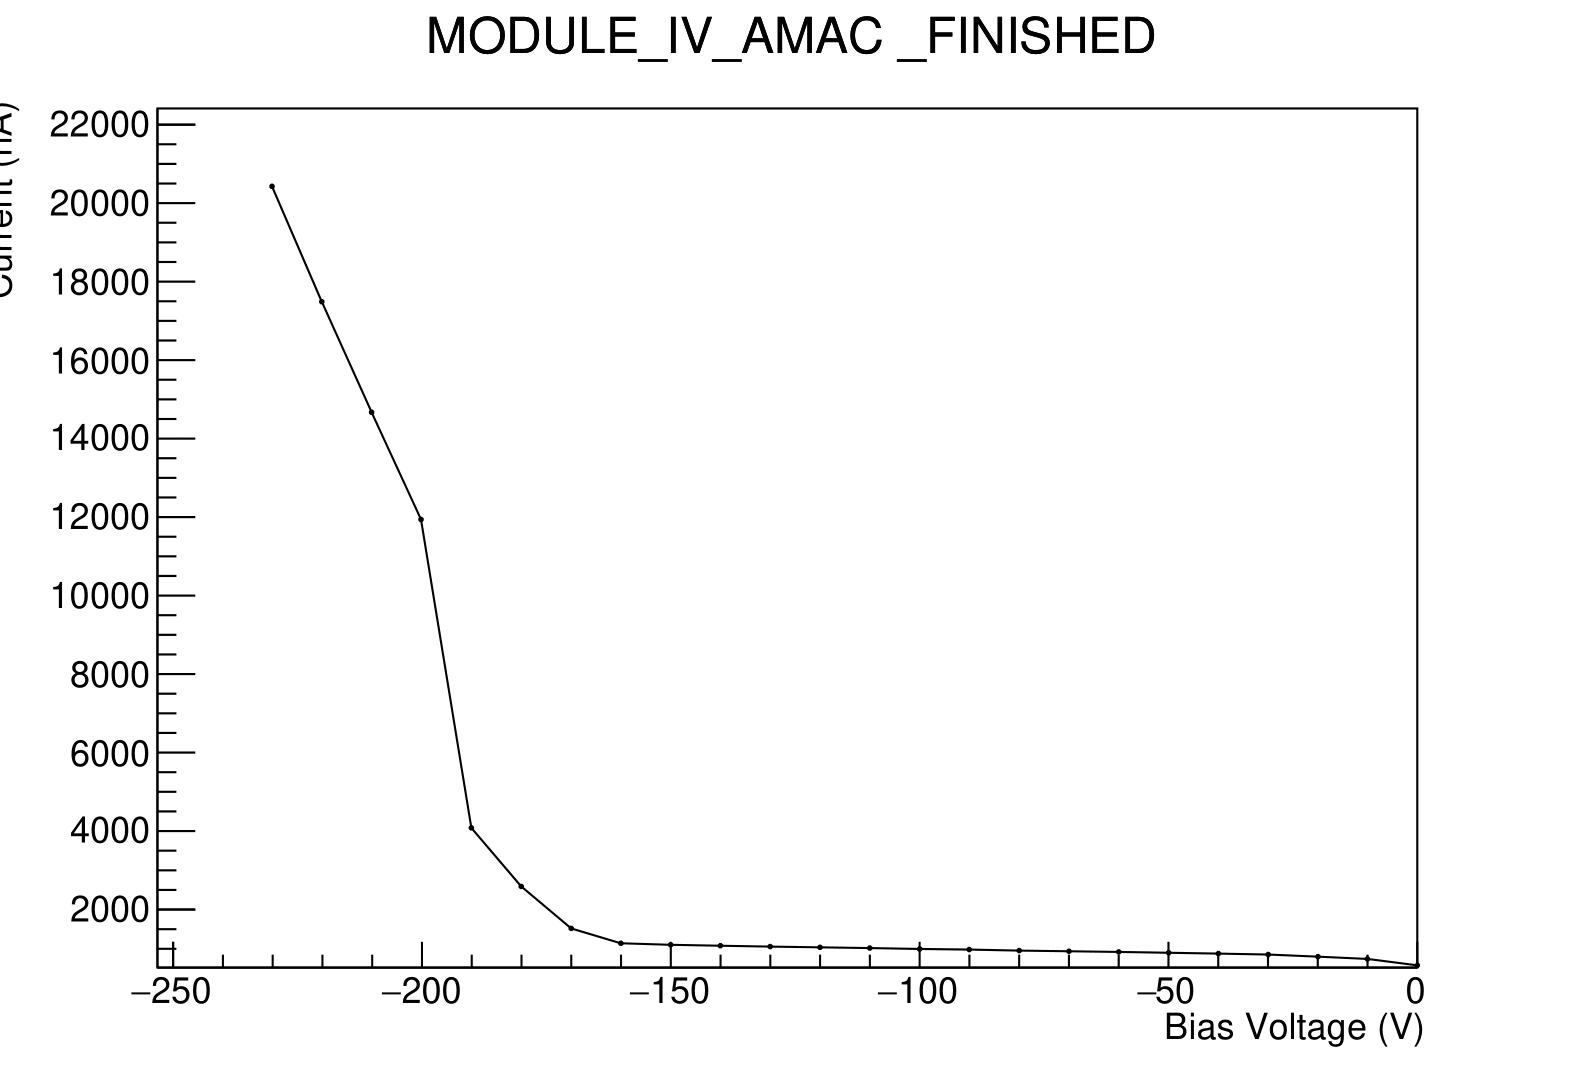
\includegraphics[width=7cm,height=8cm,keepaspectratio]{Figures/test/IV1.png}
        \caption{}\label{fig:IV1}
    \end{subfigure}
    ~
    \begin{subfigure}[b]{0.45\textwidth}
        \centering
        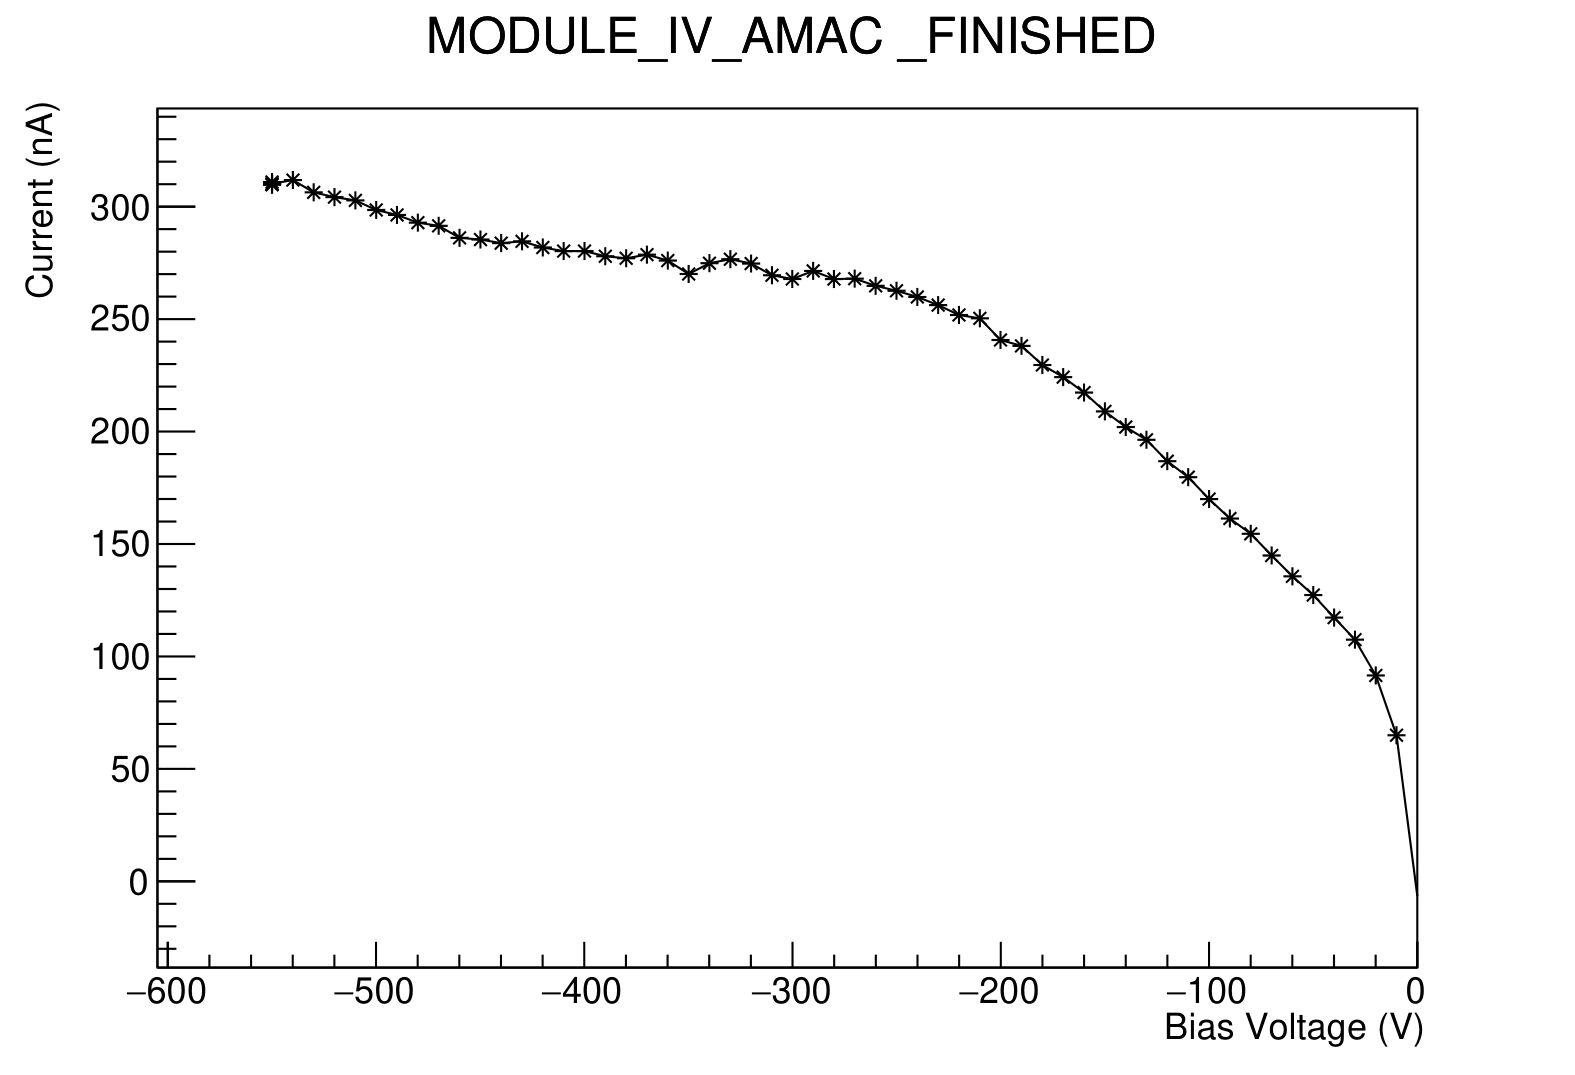
\includegraphics[width=7cm,height=8cm,keepaspectratio]{Figures/test/IV2.png}
        \caption{}\label{fig:IV2}
    \end{subfigure}
    \caption{Example plots of I-V test of a) a faulty module with a sharp breaking point of current at $-170 \si{\volt}$, and b) a healthy module with a consistent current compared to decreased voltage}
    \label{fig:IV}
\end{figure}

\textcolor{blue}{For the ITk end-cap modules, the operation voltage of $-350 \si{\volt}$ for the starting point, and the maximum of $-500 \si{\volt}$ during the late lifetime of the modules is foreseen. Consequently, we then expect a healthy module to show a consistent current without a sharp braking point within this voltage boundary in the I-V test.}







%what are each test show and why are they relevant








%Use kolanoski book